
% This LaTeX was auto-generated from an M-file by MATLAB.
% To make changes, update the M-file and republish this document.

\documentclass{article}
\usepackage{graphicx}
\usepackage{color}
\usepackage{listings}
\usepackage[framed]{mcode}
\usepackage{fullpage}
\usepackage{amsmath}
\usepackage[utf8x]{inputenc}
\usepackage{import}
\usepackage{setspace}
\usepackage{hyperref}
\definecolor{lightgray}{gray}{0.5}
\setlength{\parindent}{0pt}

\begin{document}

    
    
%\section*{}


\title{BE 521: Homework 7 \\{\normalsize p300 Speller} \\{\normalsize Spring 2021}}
\author{34 points}
\date{Due: 3/23/2021 10 PM}
\maketitle \textbf{Objective:} Spell letters using neurosignals


\begin{center} \author{Jal Mahendra Panchal}
\end{center}


\subsection*{P300 Speller}
In this homework, you will work with data from a P300-based brain computer interface called BCI2000 (Schalk et al. 2004) that allows people to spell words by focusing their attention on a particular letter displayed on the screen. In each trial the user focused on a letter, and when that letter's row or column is flashed, the user's brain elicits a P300 evoked response. By analyzing whether a P300 signal was produced, across the flashes of many different rows or columns, the computer can determine the letter that the person is focusing on.


Figure 1 shows the letter matrix from one trial of this task.
\begin{figure}
 \centering
 \includegraphics[width=0.3\textwidth]{letterMat}
 \caption{The letter matrix for the P300 speller with the third row illuminated.
          If the user were focusing on any of the letters in the third row (M, N, O, P, Q, or R),
          their brain would emit a P300 response. Otherwise it would not.}
\end{figure}


\subsection*{Data Organization}
The data for this homework is stored in \verb|I521_A0008_D001| on the IEEG Portal.
The EEG in this dataset were recorded during 85 intended letter spellings. For each letter spelling, 12 row/columns were flashed 15 times in random order ($12 \times 15 = 180$ iterations). The EEG was recorded with a sampling rate of 240 Hz on a 64-channel scalp EEG.\\


The annotations for this dataset are organized in two layers as follows:
\begin{itemize}
    \item \verb|TargetLetter| annotation layer indicates the target
    letter (annotation.description) on which the user was focusing
    during the recorded EEG segment
    (annotation.start/annotation.stop). This layer is also provided
    as TargetLetterAnnots.mat.
    \item \verb|Stim| annotation layer indicates the row/column that
    is being flashed (annotation.description) and whether the target
    letter is contained in that flash (annotation.type). The
    recorded EEG during that flash is
    (annotation.start/annotation.stop). Note that this annotation
    layer is provided as StimAnnots.mat. It is NOT on the portal.
\end{itemize}
Hints: There are many annotations in this dataset and getting them all may take ~5-10 minutes. Once you retrieve the annotations once, save them for faster loading in the future. Also, use $\verb|{ }|$ to gather variables across structs for easier manipulation (e.g. $\verb|strcmp({annotations.type},'1')|$) \\


\begin{figure}
 \centering
 \includegraphics[width=0.3\textwidth]{letterMatInds}
 \caption{The row/column indices of the letter matrix, as encoded in the \textbf{Stim} annotation layer (annotation.description) matrix.}
\end{figure}


\subsection*{Topographic EEG Maps}
You can make topographic plots using the provided \verb|topoplotEEG| function. This function needs an ``electrode file.'' and can be called like
\begin{lstlisting}
 topoplotEEG(data,'eloc64.txt','gridscale',150)
\end{lstlisting}
where \verb|data| is the value to plot for each channel. This function plots the electrodes according to the map in Figure 3.
\begin{figure}
 \centering
 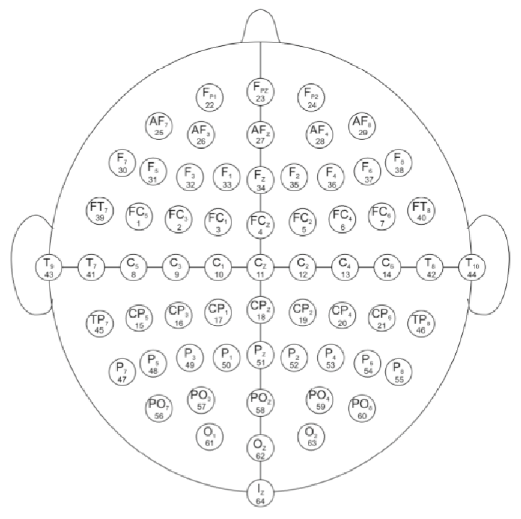
\includegraphics[width=\textwidth]{scalpEEGChans}
 \caption{The scalp EEG 64-channel layout.}
\end{figure}


\pagebreak
\section{Exploring the data}
In this section you will explore some basic properties of the data in \verb|I521_A0008_D001|.


\begin{enumerate}


 \item For channel 11 (Cz), plot the mean EEG for the target and non-target stimuli separately, (i.e. rows/columns including and not-including the desired character, respectively), on the same set of axes. Label your x-axis in milliseconds. (3 pts)

$\textbf{Answer 1.1} \\$
\begin{lstlisting}
%fetching data form the data base I521_A0008_D001
addpath(genpath('/Users/jalpanchal/git/be521'));

session = IEEGSession('I521_A0008_D001', 'jalpanchal', 'jal_ieeglogin.bin');
sampling_frequency_hz = session.data.sampleRate;
duration_in_sec = session.data(1).rawChannels(1).get_tsdetails.getDuration/1e6;

data_uV = [];
for i = 1:64
    data_uV(i,:) = session.data.getvalues(0, 15300 * 1e6, i);
end
\end{lstlisting}

\color{lightgray} \begin{lstlisting}IEEGSETUP: Adding 'ieeg-matlab.jar' to dynamic classpath
Warning: Objects of edu/upenn/cis/db/mefview/services/TimeSeriesDetails class
exist - not clearing java 
Warning: Objects of edu/upenn/cis/db/mefview/services/TimeSeriesInterface class
exist - not clearing java 
IEEGSETUP: Found log4j on Java classpath.
URL: https://www.ieeg.org/services
Client user: jalpanchal
Client password: ****
\end{lstlisting} \color{black}
\begin{lstlisting}
%load annotations
load('TargetLetterAnnots.mat')
load('StimAnnots.mat')
\end{lstlisting}
\begin{lstlisting}
%making a function to find the row/column index of a letter
letter_matrix = ['A', 'B', 'C', 'D', 'E', 'F';
                 'G', 'H', 'I', 'J', 'K', 'L';
                 'M', 'N', 'O', 'P', 'Q', 'R';
                 'S', 'T', 'U', 'V', 'W', 'X';
                 'Y', 'Z', '1', '2', '3', '4';
                 '5', '6', '7', '8', '9', '_';];

findCol = @(x) floor(find(letter_matrix==x)/6)+1;
findRow = @(x) (mod(find(letter_matrix==x),6)+6);
\end{lstlisting}
\begin{lstlisting}
%separating the trial numbers for target and non-target stimuli
target_stim_index = zeros(85,30);
nontarget_stim_index = zeros(85,150);

for i = 1:85
    target_letter = TargetLetter(i).description;
    target_row = findRow(target_letter);
    target_col = findCol(target_letter);
    temp_  = [];
    temp1_ = [];
    for j = 1:180
        stim_idx = (i-1)*180+j;
        stm_rowcol = str2double(Stim(stim_idx).description);
        if(stm_rowcol == target_row || stm_rowcol == target_col)
            temp_ = [temp_,stim_idx];
        else
            temp1_ = [temp1_,stim_idx];
        end
    end
    target_stim_index(i,:) = temp_;
    nontarget_stim_index(i,:) = temp1_;
end
\end{lstlisting}
\begin{lstlisting}
%parsing eeg data for target and nontarget trials
%Here each row represents data for 1 epoch

%each row has 240 points. This is the average of the 30 target trials
e11_target_uV = zeros(85,240);

for i = 1:85
    temp_ = [];
    temp1_ = [];
    for j = 1:30
        stm_idx = target_stim_index(i,j);
        st_idx = round(((Stim(stm_idx).start)/1e6)*sampling_frequency_hz)+1;
        sp_idx = round(((Stim(stm_idx).stop)/1e6)*sampling_frequency_hz);
        temp_ = data_uV(11,st_idx:sp_idx);
        temp1_ = [temp1_; temp_];
    end
    e11_target_uV(i,:) = mean(temp1_);
end

%each row has 240 points. This is the average of the 150 non-target trials
e11_nontarget_uV = zeros(85,240);

for i = 1:85
    temp_ = [];
    temp1_ = [];
    for j = 1:150
        stm_idx = nontarget_stim_index(i,j);
        st_idx = round(((Stim(stm_idx).start)/1e6)*sampling_frequency_hz)+1;
        sp_idx = round(((Stim(stm_idx).stop)/1e6)*sampling_frequency_hz);
        temp_ = data_uV(11,st_idx:sp_idx);
        temp1_ = [temp1_; temp_];
    end
    e11_nontarget_uV(i,:) = mean(temp1_);
end
\end{lstlisting}
\begin{lstlisting}
%Calculating the average voltage
e11_target_avg_uV = mean(e11_target_uV);
e11_nontarger_avg_uV = mean(e11_nontarget_uV);
\end{lstlisting}
\begin{lstlisting}
%plotting mean signals
t = 0 : 1/sampling_frequency_hz : 1-1/sampling_frequency_hz;
t_ms = t*1e3;

figure();
plot(t_ms, e11_target_avg_uV, 'Linewidth', 2);
hold on
plot(t_ms, e11_nontarger_avg_uV, 'Linewidth', 2);
xlabel('Time(ms)')
ylabel('Signal Amplitude(\muV)')
title('Comparing target vs non-target response for Cz channel(11)')
legend('Target', 'Non-Target')


% <latex>
%  \item Repeat the previous questions for channel 42 (T8). (1 pts)
% </latex>
\end{lstlisting}


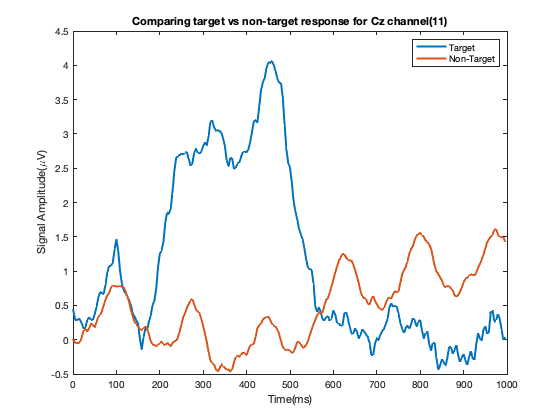
\includegraphics [width=5in]{jalp_hw7_01.png}
$\textbf{Answer 1.2} \\$
\begin{lstlisting}
%parsing eeg data for target and nontarget trials
%Here each row represents data for 1 epoch

%each row has 240 points. This is the average of the 30 target trials
e42_target_uV = zeros(85,240);

for i = 1:85
    temp_ = [];
    temp1_ = [];
    for j = 1:30
        stm_idx = target_stim_index(i,j);
        st_idx = round(((Stim(stm_idx).start)/1e6)*sampling_frequency_hz)+1;
        sp_idx = round(((Stim(stm_idx).stop)/1e6)*sampling_frequency_hz);
        temp_ = data_uV(42,st_idx:sp_idx);
        temp1_ = [temp1_; temp_];
    end
    e42_target_uV(i,:) = mean(temp1_);
end

%each row has 240 points. This is the average of the 150 non-target trials
e42_nontarget_uV = zeros(85,240);

for i = 1:85
    temp_ = [];
    temp1_ = [];
    for j = 1:150
        stm_idx = nontarget_stim_index(i,j);
        st_idx = round(((Stim(stm_idx).start)/1e6)*sampling_frequency_hz)+1;
        sp_idx = round(((Stim(stm_idx).stop)/1e6)*sampling_frequency_hz);
        temp_ = data_uV(42,st_idx:sp_idx);
        temp1_ = [temp1_; temp_];
    end
    e42_nontarget_uV(i,:) = mean(temp1_);
end
\end{lstlisting}
\begin{lstlisting}
%Calculating the average voltage
e42_target_avg_uV = mean(e42_target_uV);
e42_nontarger_avg_uV = mean(e42_nontarget_uV);
\end{lstlisting}
\begin{lstlisting}
%plotting mean signals
t = 0 : 1/sampling_frequency_hz : 1-1/sampling_frequency_hz;
t_ms = t*1e3;

figure();
plot(t_ms, e42_target_avg_uV, 'Linewidth', 2);
hold on
plot(t_ms, e42_nontarger_avg_uV, 'Linewidth', 2);
xlabel('Time(ms)')
ylabel('Signal Amplitude(\muV)')
title('Comparing target vs non-target response for T8 channel(42)')
legend('Target', 'Non-Target')
\end{lstlisting}


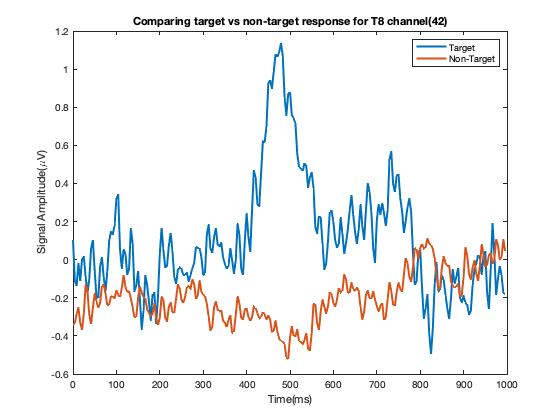
\includegraphics [width=5in]{jalp_hw7_02.png}

 \item Which of the two previous channels looks best for distinguishing between target and non-target stimuli? Which time points look best? Explain in a few sentences. (2 pts)

$\textbf{Answer 1.3} \\$
\begin{lstlisting}
e11_t_m = mean(e11_target_avg_uV);
e11_nt_m = mean(e11_nontarger_avg_uV);
snr_ratio_e11 = e11_t_m/e11_nt_m

e42_t_m = mean(e42_target_avg_uV);
e42_nt_m = mean(e42_nontarger_avg_uV);
snr_ratio_e42 = e42_t_m/e42_nt_m
\end{lstlisting}

\color{lightgray} \begin{lstlisting}
snr_ratio_e11 =

    2.2854


snr_ratio_e42 =

   -0.5591

\end{lstlisting} \color{black}
Of the channels, it looks like channel 11, Cz has a much higher ratio of Target/Non-Terget mean value as compared to the channel 42, T8. This would make it easier to detect a peak from a target stimulation in the Cz channel data. $\\$ From the graphs, in the Cz channel, we havethe highest peak at abour 450 ms which could be the best point to detect the target. While on the graph for T8 channel the peak is at about 480 ms which would be the best point to gete the target signal.

 \item Compute the mean difference between the target and non-target stimuli for each channel at timepoint 300 ms averaged across all row/column flashes. Visualize these values using the \verb|topoplotEEG| function. Include a colorbar. (3 pts)

$\textbf{Answer 1.4} \\$
\begin{lstlisting}
%calculating the mean response for each channel for all trials for all
%letters
%We'll calculate the mean of the 30 target trials for each letter/epoch.
%Then we will average the response acress each epoch to get a final 1s
%average response

all_target_avg_uV = zeros(64,240);

for e = 1:64
    temp2_ = zeros(85,240);
    for i = 1:85
        temp_ = [];
        temp1_ = [];
        for j = 1:30
            stm_idx = target_stim_index(i,j);
            st_idx = round(((Stim(stm_idx).start)/1e6)*sampling_frequency_hz)+1;
            sp_idx = round(((Stim(stm_idx).stop)/1e6)*sampling_frequency_hz);
            temp_ = data_uV(e,st_idx:sp_idx);
            temp1_ = [temp1_; temp_];
        end
        %each row has 240 points. This is the average of the 30 target trials
        temp2_(i,:) = mean(temp1_);
    end
    %Calculating avg across all 85 letters/epochs
    all_target_avg_uV(e, :) = mean(temp2_);
end

%We'll calculate the mean of the 150 non target trials for each letter/epoch.
%Then we will average the response acress each epoch to get a final 1s
%average response

all_nontarget_avg_uV = zeros(64,240);

for e=1:64
    temp2_ = zeros(85,240);
    for i = 1:85
        temp_ = [];
        temp1_ = [];
        for j = 1:150
            stm_idx = nontarget_stim_index(i,j);
            st_idx = round(((Stim(stm_idx).start)/1e6)*sampling_frequency_hz)+1;
            sp_idx = round(((Stim(stm_idx).stop)/1e6)*sampling_frequency_hz);
            temp_ = data_uV(e,st_idx:sp_idx);
            temp1_ = [temp1_; temp_];
        end
        %each row has 240 points. This is the average of the 150 non target trials
        temp2_(i,:) = mean(temp1_);
    end
    %Calculating avg across all 85 letters/epochs
    all_nontarget_avg_uV(e, :) = mean(temp2_);
end
\end{lstlisting}
\begin{lstlisting}
%Calculating the difference betweeen target and non target signals at
%300 ms. The 73rd data point contain data from 300-304.167 ms
diff_at300_uV = (all_target_avg_uV(:,73))-(all_nontarget_avg_uV(:,73));
\end{lstlisting}
\begin{lstlisting}
%Plotting target-nontarget values at 300ms
figure();
cmap = colormap(jet);
topoplotEEG(diff_at300_uV,'eloc64.txt','gridscale', 150, 'colormap', cmap, 'electrodes', 'numbers')
h = colorbar;
title('Difference in uV between target and non-taregt stimuli at 300 ms')
\end{lstlisting}

\color{lightgray} \begin{lstlisting}  Name       Size            Bytes  Class     Attributes

  x         64x1               512  double              
  y         64x1               512  double              

\end{lstlisting} \color{black}


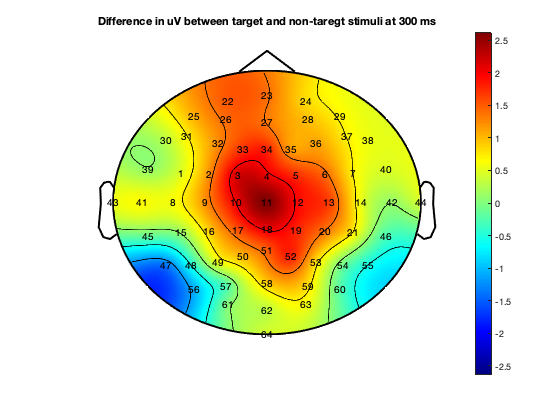
\includegraphics [width=5in]{jalp_hw7_03.png}

 \item How do the red and blue parts of this plot correspond to the plots from above? (2 pts)

$\textbf{Answer 1.5} \\$
In the color bar chosen, red color signifies the largest difference between the target and non-tartet response at those electrode locations. The blue color in the other hand shows areas where the non-target stimuli have a greater response as compared to the target stimuli. Or it could also be locations where the target response as more negative as compared to the non-target response. $\\$ Here we see that the Cz electrode has the highest difference while the T8 electrode has a very small difference between the target and non-target respose at 300ms. This is consistent with the plots in 1.1and 1.2 where we observed a might higher ratio and difference in Cz as compared to T8 electrode.

\end{enumerate}
\section{Using Individual P300s in Prediction}
Hopefully the Question 1.4 convinced you that the Cz channel is a reasonably good channel to use in separating target from non-target stimuli in the P300. For the rest of the homework, you will work exclusively with this channel.
\begin{enumerate}
 \item Explain a potential advantage to using just one channel other than the obvious speed of calculation advantage. Explain one disadvantage. (3 pts)

$\textbf{Answer 2.1} \\$
By just using one channel we can simplify the hardware and usability of the whole system as then only 2 electrodes (cz and ground) will be needed for the prediction. This is help with storage, power and computational needs. $\\$ One big disadvantage of using 1 electrode is it does not help adapt to people who have disabilities in the brain or have imapairment/damage. We would then now know if the region detected by the Cz electrode is the the right one. For some people due to neuroplasticity their area of high activity might be different than the one detected by Cz. In all of these cases it would make more sense to have the complete skull covered instead of a single or only a few electrodes.

 \item One simple way of identifying a P300 in a single trial (which we'll call the \emph{p300 score}) is to take the mean EEG from 250 to 450 ms and then subtract from it the mean EEG from 600 to 800 ms. What is the 	\emph{p300 score} for epoch (letter) 10, iteration 11 at electrode Cz? (3 pts)

$\textbf{Answer 2.2} \\$
\begin{lstlisting}
%Calculating pscore for Cz channel
%250ms to 450 ms is at index 61 to 108
%600 to 800 ms is from index 145-192

pscore_c11 = zeros(85,180);

for i = 1:85
    for j = 1:180
        %separatingindex for each trial in each epoch
        stim_idx = (i-1)*180+j;
        %finding the index fro the datafrom time stamps
        st_idx = round(((Stim(stim_idx).start)/1e6)*sampling_frequency_hz)+1;
        sp_idx = round(((Stim(stim_idx).stop)/1e6)*sampling_frequency_hz);
        temp_ = data_uV(11,st_idx:sp_idx);

        %pscore = val(250-450)ms-val(600to800)
        pscore_c11(i,j) = mean(temp_(61:108))-mean(temp_(145:192));
    end
end
\end{lstlisting}
\begin{lstlisting}
%pscore for epoch 10 and iterarion 11 is
pscore_c11(10,11)
\end{lstlisting}

\color{lightgray} \begin{lstlisting}
ans =

    0.8243

\end{lstlisting} \color{black}
The $pscore$ for epoch 10 and iteration 11 at electrode Cz is 0.8243

 \item Plot the \emph{p300 scores} for each row/column in epoch 27 at electrode Cz. (3 pts)

$\textbf{Answer 2.3} \\$
\begin{lstlisting}
%first we must find the indexes of the 15 trials for each row and column

epoch27_stim_rowcol = zeros(1,180);
for i = 1:180
    epoch27_stim_rowcol(i) = str2double(Stim(26*180+i).description);
end

%separate the indexes for ech row and col number creating a 12x15 index
%table
epoch_27_idx_separated = zeros(12,15);
pscore_c11_separated = zeros(12,15);
for i = 1:12
    epoch_27_idx_separated(i, :) = find(epoch27_stim_rowcol==i);
    pscore_c11_separated(i,:) = pscore_c11(27, epoch_27_idx_separated(i, :));
end
\end{lstlisting}
\begin{lstlisting}
%boxplot for all iterations of each row/column
figure();
boxplot(pscore_c11_separated')
ylabel('p300 score (\muV)')
xlabel('Row/Column Number')
title('p300 score value across trials for each row/column at Cz, epoch 27')
\end{lstlisting}


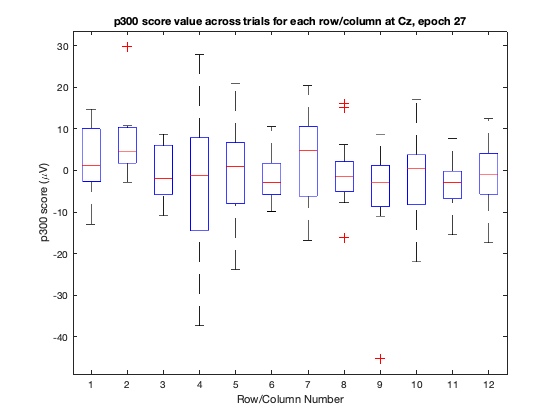
\includegraphics [width=5in]{jalp_hw7_04.png}

 \item Based on your previous answer for epoch 27, what letter do you predict the person saw? Is this prediction correct? (2 pts)

$\textbf{Answer 2.4} \\$
Based the values from 2.3, we see that the Column \#2 and Row \#7 have the highest mean. When we see the intersection of the 2 values, the letter is B. This matches the epoch 27 in the TargetLetter annotation.

 \item Using this \emph{p300 score}, predict (and print out) the letter viewed at every epoch. What was you prediction accuracy? (2 pts)

$\textbf{Answer 2.5} \\$
\begin{lstlisting}
%Calculating the p300 score for all epochs
pscore_c11_allepoch = zeros(85,12);

for i = 1:85
    epoch_i_stim_rowcol = zeros(1,180);
    for j = 1:180
        epoch_i_stim_rowcol(j) = str2double(Stim((i-1)*180+j).description);

    end

    %separate the indexes for each row and col number creating a 12x15 index
    %table
    epoch_i_idx_separated = zeros(12,15);
    pscore_temp_ = zeros(12,15);
    for k = 1:12
        epoch_i_idx_separated(k, :) = find(epoch_i_stim_rowcol==k);
        pscore_temp_(k,:) = pscore_c11(i, epoch_i_idx_separated(k, :));
    end

    %calculating the average p300 score across all 15 trails for each
    %row/col
    temp_ = mean(pscore_temp_,2);
    pscore_c11_allepoch(i,:)= temp_';
end
\end{lstlisting}
\begin{lstlisting}
%finding the predicted letter in each epoch
%We'll find the row/col with the 2 highest p300 scores
%find the intersection of the row and column to find the predicted letter

c11_p300_accuracy = zeros(1,85);
for i = 1:85

    %find index for row and col with 2 highest p300 values
    [~,temp_idx] = sort(pscore_c11_allepoch(i,:), 'descend');

    %parsing row and column index
    %finding highest row index
    temp1_  = find(temp_idx>6);
    row_idx = temp_idx(temp1_(1))-6;

    %finding highest column index
    temp2_  = find(temp_idx<7);
    col_idx = temp_idx(temp2_(1));

    pred_letter = letter_matrix(row_idx,col_idx)
    target_letter = TargetLetter(i).description

    c11_p300_accuracy(i) = pred_letter==TargetLetter(i).description;
end


prediction_accuracy = sum(c11_p300_accuracy)/85*100
\end{lstlisting}

\color{lightgray} \begin{lstlisting}
pred_letter =

    '4'


target_letter =

    'E'


pred_letter =

    'A'


target_letter =

    'A'


pred_letter =

    '8'


target_letter =

    'E'


pred_letter =

    'V'


target_letter =

    'V'


pred_letter =

    'E'


target_letter =

    'Q'


pred_letter =

    'U'


target_letter =

    'T'


pred_letter =

    'F'


target_letter =

    'D'


pred_letter =

    'O'


target_letter =

    'O'


pred_letter =

    '8'


target_letter =

    'J'


pred_letter =

    'I'


target_letter =

    'G'


pred_letter =

    'O'


target_letter =

    '8'


pred_letter =

    'W'


target_letter =

    'R'


pred_letter =

    'B'


target_letter =

    'B'


pred_letter =

    'M'


target_letter =

    'R'


pred_letter =

    'J'


target_letter =

    'G'


pred_letter =

    'O'


target_letter =

    'O'


pred_letter =

    'F'


target_letter =

    'N'


pred_letter =

    'C'


target_letter =

    'C'


pred_letter =

    'F'


target_letter =

    'E'


pred_letter =

    'D'


target_letter =

    'D'


pred_letter =

    '9'


target_letter =

    'H'


pred_letter =

    'C'


target_letter =

    'C'


pred_letter =

    'T'


target_letter =

    'T'


pred_letter =

    'X'


target_letter =

    'U'


pred_letter =

    'I'


target_letter =

    'I'


pred_letter =

    'D'


target_letter =

    'D'


pred_letter =

    'B'


target_letter =

    'B'


pred_letter =

    '6'


target_letter =

    'P'


pred_letter =

    'U'


target_letter =

    'U'


pred_letter =

    '1'


target_letter =

    'H'


pred_letter =

    'A'


target_letter =

    'M'


pred_letter =

    'W'


target_letter =

    'E'


pred_letter =

    'R'


target_letter =

    'M'


pred_letter =

    '5'


target_letter =

    '6'


pred_letter =

    'I'


target_letter =

    'O'


pred_letter =

    'O'


target_letter =

    'U'


pred_letter =

    'K'


target_letter =

    'X'


pred_letter =

    'O'


target_letter =

    'O'


pred_letter =

    'I'


target_letter =

    'C'


pred_letter =

    'Q'


target_letter =

    'F'


pred_letter =

    'O'


target_letter =

    'O'


pred_letter =

    'O'


target_letter =

    'U'


pred_letter =

    'C'


target_letter =

    'K'


pred_letter =

    'X'


target_letter =

    'W'


pred_letter =

    'E'


target_letter =

    'A'


pred_letter =

    '_'


target_letter =

    '4'


pred_letter =

    'T'


target_letter =

    'V'


pred_letter =

    'G'


target_letter =

    'J'


pred_letter =

    'K'


target_letter =

    'E'


pred_letter =

    '4'


target_letter =

    'F'


pred_letter =

    'R'


target_letter =

    'R'


pred_letter =

    '2'


target_letter =

    'Z'


pred_letter =

    '3'


target_letter =

    'R'


pred_letter =

    'G'


target_letter =

    'O'


pred_letter =

    'L'


target_letter =

    'L'


pred_letter =

    'H'


target_letter =

    'H'


pred_letter =

    'Y'


target_letter =

    'Y'


pred_letter =

    '6'


target_letter =

    'N'


pred_letter =

    'Q'


target_letter =

    'Q'


pred_letter =

    '_'


target_letter =

    'D'


pred_letter =

    'K'


target_letter =

    'W'


pred_letter =

    'X'


target_letter =

    '_'


pred_letter =

    'E'


target_letter =

    'E'


pred_letter =

    '9'


target_letter =

    'K'


pred_letter =

    'V'


target_letter =

    'T'


pred_letter =

    'L'


target_letter =

    'L'


pred_letter =

    'R'


target_letter =

    'B'


pred_letter =

    'X'


target_letter =

    'W'


pred_letter =

    'T'


target_letter =

    'X'


pred_letter =

    'K'


target_letter =

    'E'


pred_letter =

    'K'


target_letter =

    'P'


pred_letter =

    'P'


target_letter =

    'O'


pred_letter =

    'I'


target_letter =

    'U'


pred_letter =

    'H'


target_letter =

    'I'


pred_letter =

    'N'


target_letter =

    'K'


pred_letter =

    'G'


target_letter =

    'Z'


pred_letter =

    'F'


target_letter =

    'E'


pred_letter =

    '4'


target_letter =

    'R'


pred_letter =

    'L'


target_letter =

    'Y'


pred_letter =

    'L'


target_letter =

    'O'


pred_letter =

    'U'


target_letter =

    'O'


pred_letter =

    '5'


target_letter =

    'T'


pred_letter =

    'B'


target_letter =

    'H'


pred_letter =

    'Q'


target_letter =

    'Q'


pred_letter =

    'R'


target_letter =

    'I'


prediction_accuracy =

   27.0588

\end{lstlisting} \color{black}
The prediction accuracy by using the highest p300 values for rows and columns trials and finding the intersection of the 2 is 27.06\%.

\end{enumerate}
\section{Automating the Learning}
In Section 2, you used a fairly manual method for predicting the letter. Here, you will have free rein to use put any and all learning techniques to try to improve your testing accuracy.
\begin{enumerate}
 \item Play around with some ideas for improving/generalizing the prediction paradigm used in the letter prediction. Use the first 50 letter epochs as the training set and the later 35 for validation. Here, you are welcome to hard-code in whatever parameters you like/determine to be optimal. What is the optimal validation accuracy you get? Note: don't worry too much about accuracy, we are more interested in your thought process. (4 pts)

$\textbf{Answer 3.1} \\$
To improve the prediction from section 2, we will include 9 electrodes in the analysis. Cz and the 8 electrodes surrounding it.  We will then calculate a average p300 score from the 9 electrodes. We will also extend the timing range for p300 calculation to 250-500 ms.
\begin{lstlisting}
%Extending the timimng for p300 to 250-500ms
%Calculating average p300score for 9 channels
%250ms to 500 ms is at index 61 to 120
%600 to 800 ms is from index 145-192

%channels 3,4,5,10,11,12,17,18,19
%the choosen channels are the 8 channels around channel 11,Cz
electrode_arr = [3,4,5,10,11,12,17,18,19];


%we'll now caculate the average p300 score for the 9 electrodes

p300score_nineavg = zeros(85,180);

for i = 1:85
    for j = 1:180

        %separatingindex for each trial in each epoch
        stim_idx = (i-1)*180+j;
        %finding the index fro the datafrom time stamps
        st_idx = round(((Stim(stim_idx).start)/1e6)*sampling_frequency_hz)+1;
        sp_idx = round(((Stim(stim_idx).stop)/1e6)*sampling_frequency_hz);

        p300_temp_ = zeros(9,1);
        for e = 1:9
            temp_ = data_uV(electrode_arr(e),st_idx:sp_idx);

            %p300 score = val(250-500)ms-val(600to800)
            p300_temp_(e) = mean(temp_(61:120)-mean(temp_(145:192)));
        end

        %calculating mean p300 value
        mean_temp_ = mean(p300_temp_);

        %p300 score = val(250-500)ms-val(600to800)
        p300score_nineavg(i,j) = mean_temp_;
    end
end
\end{lstlisting}
\begin{lstlisting}
%Calculating the mean p300 score for 12 rows and columns
%Calculating the mean p300 score for all epochs
p300score_stimavg = zeros(85,12);

for i = 1:85
    epoch_i_stim_rowcol = zeros(1,180);
    for j = 1:180
        epoch_i_stim_rowcol(j) = str2double(Stim((i-1)*180+j).description);

    end

    %separate the indexes for each row and col number creating a 12x15 index
    %table
    epoch_i_idx_separated = zeros(12,15);
    pscore_temp_ = zeros(12,15);
    for k = 1:12
        epoch_i_idx_separated(k, :) = find(epoch_i_stim_rowcol==k);
        pscore_temp_(k,:) = p300score_nineavg(i, epoch_i_idx_separated(k, :));
    end

    %calculating the average p300 score across all 15 trails for each
    %row/col
    temp_ = mean(pscore_temp_,2);
    p300score_stimavg(i,:)= temp_';
end
\end{lstlisting}
Now we have the average p300 for each of the 12 stim row/cols for each epoch. We will train a classifier for the rows and column index separately. To do this, for each epoch, we will create a 2 sets of features, the p300 score for a row and a p300 score for a column. We will then create separate SVM models to predict the correct row and column. for each epoch we will have 6 data points for each feature.
\begin{lstlisting}
%we will first normalize across each epoch
p300score_stimavg_norm = normalize(p300score_stimavg')';

%separating row and columns data
p300_rows = p300score_stimavg_norm(:,7:12);
p300_cols = p300score_stimavg_norm(:,1:6);

%separating training and testing data
p300_rows_train = p300_rows(1:50,:);
p300_rows_test = p300_rows(51:85,:);

p300_cols_train = p300_cols(1:50,:);
p300_cols_test = p300_cols(51:85,:);

%converting into a column matrix
p300_rows_train_vec = reshape(p300_rows_train,[],1);
p300_rows_test_vec = reshape(p300_rows_test, [],1);

p300_cols_train_vec = reshape(p300_cols_train, [],1);
p300_cols_test_vec = reshape(p300_cols_test, [],1);
\end{lstlisting}
\begin{lstlisting}
%creating the labels for training and validation
all_labels = zeros(85,12);

for i = 1:85
    target_letter = TargetLetter(i).description;
    tar_row = findRow(target_letter);
    tar_col = findCol(target_letter);
    all_labels(i,tar_col) = 1;
    all_labels(i,tar_row) = 1;
end

row_labels_train = reshape(all_labels(1:50,7:12), [],1);
col_labels_train = reshape(all_labels(1:50,1:6), [],1);
\end{lstlisting}
\begin{lstlisting}
%using a SVM classifier
%for rows
X = p300_rows_train_vec;
Y = row_labels_train;

svmodel_rows = fitcsvm(X,Y, 'KernelFunction','rbf')

%Calculating training error by predicting the training set
row_pred_train_svm = predict(svmodel_rows, X);

train_error_svm_rows = size(find(row_pred_train_svm~=Y),1)/size(Y,1)
\end{lstlisting}

\color{lightgray} \begin{lstlisting}
svmodel_rows = 

  ClassificationSVM
             ResponseName: 'Y'
    CategoricalPredictors: []
               ClassNames: [0 1]
           ScoreTransform: 'none'
          NumObservations: 300
                    Alpha: [89×1 double]
                     Bias: -0.6493
         KernelParameters: [1×1 struct]
           BoxConstraints: [300×1 double]
          ConvergenceInfo: [1×1 struct]
          IsSupportVector: [300×1 logical]
                   Solver: 'SMO'



train_error_svm_rows =

    0.1233

\end{lstlisting} \color{black}
\begin{lstlisting}
%SVM classifier for columns
X = p300_cols_train_vec;
Y = col_labels_train;

svmodel_cols = fitcsvm(X,Y, 'KernelFunction','rbf')

%Calculating training error by predicting the training set
cols_pred_train_svm = predict(svmodel_cols, X);

train_error_svm_cols = size(find(cols_pred_train_svm~=Y),1)/size(Y,1)
\end{lstlisting}

\color{lightgray} \begin{lstlisting}
svmodel_cols = 

  ClassificationSVM
             ResponseName: 'Y'
    CategoricalPredictors: []
               ClassNames: [0 1]
           ScoreTransform: 'none'
          NumObservations: 300
                    Alpha: [98×1 double]
                     Bias: -0.5212
         KernelParameters: [1×1 struct]
           BoxConstraints: [300×1 double]
          ConvergenceInfo: [1×1 struct]
          IsSupportVector: [300×1 logical]
                   Solver: 'SMO'



train_error_svm_cols =

    0.1367

\end{lstlisting} \color{black}
To complete the prediction, we will check the classification of the model for the set of 6 rows and cols. If the model returns a 1, then that row/col is selected. If No row/col is classified at valid, we'll choose the one with the highest p300 value. If more than one row/cal are classified, we'll choose the one with the highest p300 value.
\begin{lstlisting}
%testing/validating the models

testing_accuracy_svm = zeros(1,35);
for i = 1:35

    %predicting row_index
    test_pred_row_val = predict(svmodel_rows, p300_rows_test(i,:)');

    if sum(test_pred_row_val) ==0
        [~,pred_row] = max(p300_rows_test(i,:));
    elseif sum(test_pred_row_val) > 1
        temp_ = max(p300_rows_test(i,test_pred_row_val==1));
        pred_row  = find(p300_rows_test(i,:)==temp_);
    else
        [pred_row] = find(test_pred_row_val==1);
    end


    %Predicting column index
    test_pred_col_val = predict(svmodel_cols, p300_cols_test(i,:)');

    if sum(test_pred_col_val) ==0
        [~,pred_col] = max(p300_cols_test(i,:));
    elseif sum(test_pred_col_val) > 1
        temp_ = max(p300_cols_test(i,test_pred_col_val==1));
        pred_col  = find(p300_cols_test(i,:)==temp_);
    else
        pred_col = find(test_pred_col_val==1);
    end

    pred_letter = letter_matrix(pred_row,pred_col)

    testing_accuracy_svm(i) = pred_letter ==TargetLetter(i).description;

end

testing_accuracy = sum(testing_accuracy_svm)/35*100
\end{lstlisting}

\color{lightgray} \begin{lstlisting}
pred_letter =

    'R'


pred_letter =

    '2'


pred_letter =

    '3'


pred_letter =

    'G'


pred_letter =

    'L'


pred_letter =

    'H'


pred_letter =

    '1'


pred_letter =

    '6'


pred_letter =

    'O'


pred_letter =

    'F'


pred_letter =

    'W'


pred_letter =

    'W'


pred_letter =

    'A'


pred_letter =

    '9'


pred_letter =

    'V'


pred_letter =

    'L'


pred_letter =

    'P'


pred_letter =

    'X'


pred_letter =

    'T'


pred_letter =

    'E'


pred_letter =

    'K'


pred_letter =

    '2'


pred_letter =

    '7'


pred_letter =

    'H'


pred_letter =

    'N'


pred_letter =

    'Z'


pred_letter =

    'F'


pred_letter =

    'X'


pred_letter =

    'L'


pred_letter =

    'L'


pred_letter =

    'U'


pred_letter =

    'T'


pred_letter =

    'B'


pred_letter =

    'Q'


pred_letter =

    'L'


testing_accuracy =

     0

\end{lstlisting} \color{black}
I tried tuning the model quite a bit but could not make the algorithm predict the letters well.

 \item Describe your algorithm in detail. Also describe what you tried that didn't work. (6 pts)

$\textbf{Answer 3.2} \\$
The steps followed in the algorithm above : \ensuremath{\backslash}begin\{enumerate\} \ensuremath{\backslash}item To begin with, to improve the prediction from section 2, I included 9 electrodes in the analysis. Cz and the 8 electrodes surrounding it. I then calculate a average p300 score from the 9 electrodes. I also extended the timing range for p300 calculation to 250-500 ms. \ensuremath{\backslash}item For each trial I calculate the p300 value for all 9 electrodes and then calculate a mean value of the p300 from the 9 electrodes \ensuremath{\backslash}item I then calaculate the average p300 for he 15 trials of each of the 12 rows/columns giving a 85x12 matrix of mean p300 values \ensuremath{\backslash}item I then normalize the p300 values for each epoch \ensuremath{\backslash}item the I separate the p300 values for the row and column triggers. \ensuremath{\backslash}item The 85x6 matrices for the rows and columns are then split into the 50 training ans the the 35 testing set. \ensuremath{\backslash}item The training set for rows and columsn is convereted from a 50x6 matrix to a 300x1 column vector so that each row/column can be classified as a valied p300 or not \ensuremath{\backslash}item this 300x1 vector of p300 values for rows is used to train a SVM model with gaussian kernal. The same is dont for a model using the column values of p300. the calssification on both cases is binary with a 1 given to the right row/column and a 0 to a non-target row/column. \ensuremath{\backslash}item The model is then used to predict data from a new epock by predicting a row or column value. \ensuremath{\backslash}item If the model classisifies more than one row/column as a valied p300 them the one with the higher p300 is chooson. If the model does not classify any row/column as a valid p300 then the value with the hihghest p300 for the epock is choosen. For testing I followed the same averaging process as training using the 9 electrodes and averaging the 15 trials for each row/column. \ensuremath{\backslash}end\{enumerate\}
Other methods tried : \ensuremath{\backslash}begin\{enumerate\} \ensuremath{\backslash}item I calculated the p300 scrore using the ratio of values from 250-500 ms to those from 600-800 ms. The ratio was created a lot of anomolies due to the decimal and negetive values in teh data \ensuremath{\backslash}item I tried the model using only cZ and using more electrodes to give the same result \ensuremath{\backslash}item I also tried averaging the siganl across the electrodes and then calculating the p300 values \ensuremath{\backslash}item I also tried using fitcecoc to train a multiclass classifier to classify the p300 values for rows and columns in 6 classes \ensuremath{\backslash}end\{enumerate\}

\end{enumerate}
\end{document}




\end{document}
    
